
In this chapter, we use the following steady-state case of single-phase porous media flow to 
illustrate a popular method of model order reduction, namely, the proper orthogonal decomposition 
method.
\section{MOR for steady-state problem}
\subsection{Model order reduction by POD}
\begin{itemize}
\item Model equations
\begin{equation} \label{single-phase}
\left\{
\begin{aligned}
- \nabla \cdot (\kappa \nabla p) & = 0  \qquad \text{in}~~ \Omega \\
\kappa \nabla p \cdot n &= f \qquad \text{on} ~~ \Gamma_\text{N} \\
p  &= 0 \qquad \text{on} ~~\Gamma_{\text{D}1} \\
p  &= 1 \qquad \text{on}~~ \Gamma_{\text{D}2} 
\end{aligned}
\right. 
\end{equation}
\begin{center}
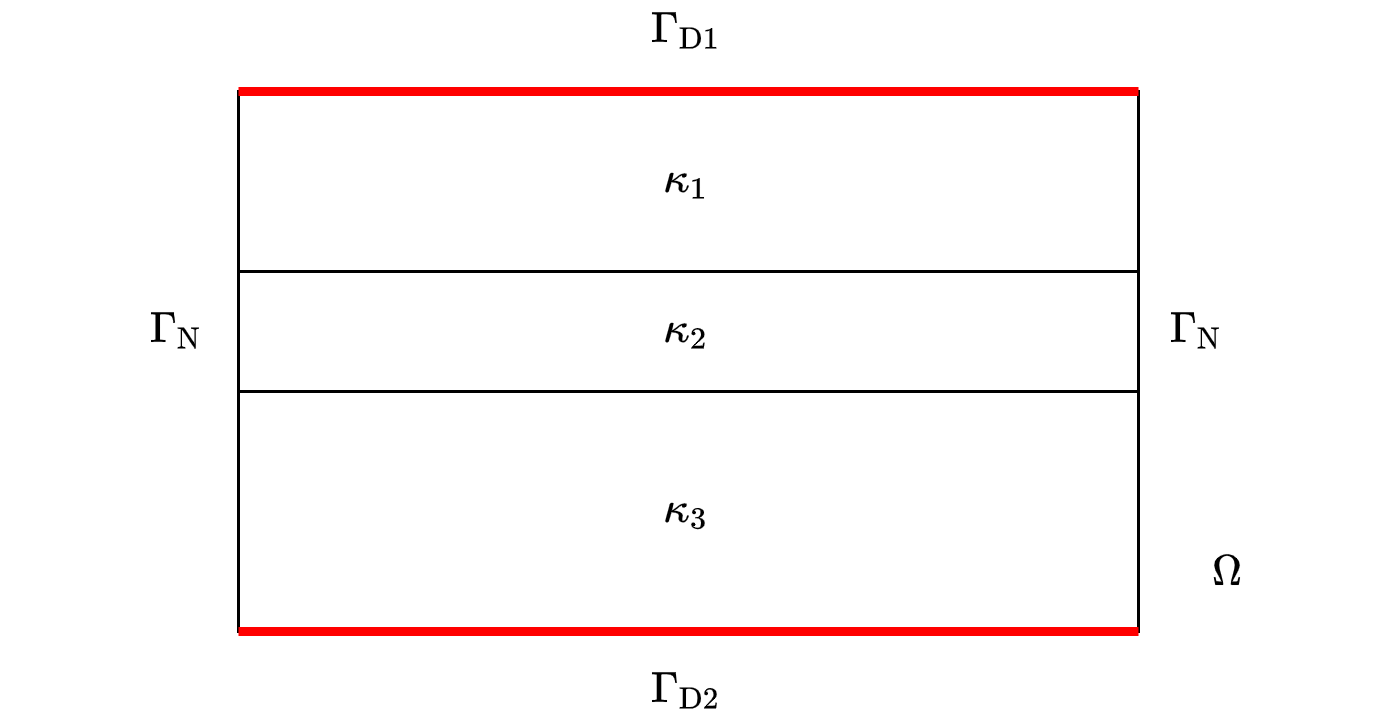
\includegraphics[height=3.5cm]{figures/RBM/Darcy_domain.png}
\end{center}
\item In history matching, we need to solve the equations \eqref{single-phase} many times with different $\kappa$. Can we reuse the solution obtained in the process to reduce computational cost for the future?
\end{itemize}

\begin{figure}[!ht]
\begin{center}
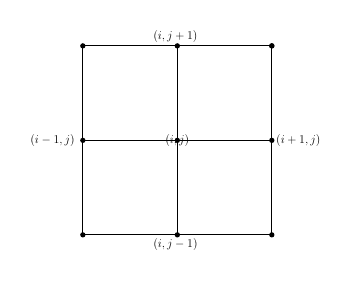
\begin{tikzpicture}[xscale=1.2,yscale=1.2]
\tikzstyle{every node}=[font=\Large,scale=0.3]
\draw[-] (3,0) -- (5,0);
%\draw[-] (3,0.5) -- (5,0.5);
\draw[-] (3,1) -- (5,1);
%\draw[-] (3,1.5) -- (5,1.5);
\draw[-] (3,2) -- (5,2);

\draw[-] (3,0) -- (3,2);
%\draw[-] (3.5,0) -- (3.5,2);
\draw[-] (4,0) -- (4,2);
%\draw[-] (4.5,0) -- (4.5,2);
\draw[-] (5,0) -- (5,2);

\node at (4.00,1) {${\red {\tiny{(i,j)}}}$};
\node at (5.28,1) {${\red {\tiny{(i+1,j)}}}$};
\node at (5.18,2) {};%{${\red {0}}$}
\node at (5.18,0){};% {${\red {0}}$}
\node at (2.68,1) {${\red {\tiny{(i-1,j)}}}$};
\node at (2.78,2) {};%{${\red {0}}$}

\node at (2.78,0){};%{${\red {0}}$}

\node at (3.98, 2.1) {${\red {\tiny{(i,j+1)}}}$};
\node at (3.98, -0.1) {${\red {\tiny{(i,j-1)}}}$};

\fill(5,2) circle(0.8pt);
\fill(4,2) circle(0.8pt);
\fill(3,2) circle(0.8pt);
\fill(3,1) circle(0.8pt);
\fill(4,1) circle(0.8pt);
\fill(5,1) circle(0.8pt);
\fill(5,0) circle(0.8pt);
\fill(5,2) circle(0.8pt);
\fill(3,0) circle(0.8pt);
\fill(4,0) circle(0.8pt);
\end{tikzpicture}
\end{center}
\end{figure}

Five-point stencil finite difference scheme of the model \eqref{single-phase}
reads (if $\kappa \equiv 1$):  
$$
\frac{4p_{i,j}-p_{i,j-1}-p_{i,j+1}-p_{i+1,j}-p_{i-1,j}}{h^2}=f_{i,j} \quad 1 \le i,j \le n;
$$
In practice, there are many details to look into, for example, complex geometry, 
boundary conditions, general coefficient $\kappa$,  and mass conservation.
We can also use other discretization methods, like FVM, FEM, DG, and so on. 

Let $d=n^2$ and $x_{\kappa}\in \mathbb R^d$ be the solution vector, i.e., 
$$
x_{\kappa, (i-1)n+j} := p_{i,j}, \qquad 1 \le i \le n,  1 \le j \le n.
$$
\begin{center}
\includegraphics[height=3.5cm]{figures/RBM/2Dto1Dordering.png}
\end{center}
In the end, we need to solve a linear system
\begin{equation}
A_{\kappa}x_{\kappa} = b_{\kappa},\quad  x_{\kappa}\in \mathbb{R}^d.
\end{equation}
We need to solve very large linear systems  and the computational cost is expensive.
Hence, we want to reuse the computed solutions to help obtaining solution for a new parameter.
The basic Idea is constructing a reduced model based on the available solutions of the original full model to get accurate approximations. 

\paragraph{Obtain training data}
Pick $N$ samples $\kappa_\ell \in \mathcal{D}, \ell=1, 2, \ldots, N$, where $\mathcal{D}$ is a compact set for the parameters. For each $\kappa_\ell$, we solve for $x_\ell:=x_{\kappa_\ell}$ such that
$$
A_{\ell} \, x_\ell = b_{\ell}.
$$
Then we have 
$$
X = \Big[ x_1,x_2, \ldots, x_N \Big] \in \mathbb{R}^{d\times N}.
$$
Denote $\bar{x} = \frac{1}{N}\sum_{\ell=1}^{N} x_{\ell}$ and 
$$
\overline{X} = \Big[\bar{x},\bar{x}, \ldots, \bar{x} \Big] \in \mathbb{R}^{d\times N}.
$$
In practice, we may collect the already computed solutions as $X$.

\paragraph{POD: proper orthogonal decomposition}

\begin{itemize}\setlength{\itemsep}{10pt}
\item Eigen-decomposition: $$(X-\overline{X})(X-\overline{X})^T=W \Sigma W^T=\sum_{i=1}^d \sigma^2_i w_i w_i^T$$

where $W=[w_1,...,w_d]$, $W^TW=I$.
\item Eigenvalues of $(X-\overline{X})(X-\overline{X})^T$: 
$$
\sigma_1^2 \ge \sigma_2^2 \ge \cdots \ge \sigma^2_{d'}\gg  \sigma^2_{d'+1}\ge \cdots\ge \sigma^2_d
$$
\item Obtain an orthogonal reduced basis
$$
\hat W=[w_1,w_2,\cdots,w_{d'}].
$$
\end{itemize}

\paragraph{Model reduction for steady-state problem}


\begin{itemize}\setlength{\itemsep}{10pt}

\item PCA: $y_\kappa=\hat{W}\hat{W}^T(x_\kappa-\bar{x})+\bar{x} = g \circ f \, (\hat x_{\kappa})$
\item Encoder $\hat{x}=f(x) = \hat{W}^T(x-\bar{x})$ 
\item Decoder $g(\hat{x})=W\hat{x}+\bar{x}$ 
\item Encode the original equation 
$
f(A_\kappa x_\kappa)=f(b_\kappa) \Leftrightarrow \hat W^T A_\kappa x_\kappa=\hat W^Tb_\kappa
$
\item Approximate $x_\kappa\approx y_\kappa=\hat{W}\hat{W}^T(x_\kappa-\bar{x})+\bar{x}$
	$$\hat W^T A_\kappa y_\kappa=\hat W^Tb_\kappa,$$
	which is
		
		\begin{center}
		$
		\hat W^T A_\kappa \hat{W} (\hat{W}^T(x_\kappa-\bar{x}))=\hat W^T(b_\kappa - A_{\kappa}\bar{x})
		$
		\end{center}
		
\item Noting that $\hat{x_\kappa} = f(x_\kappa) = \hat{W}^T(x_\kappa-\bar{x})$. So we obtain that
		$$
		\hat W^T A_\kappa \hat{W} \hat{x_\kappa} =\hat W^T(b_\kappa - A_{\kappa}\bar{x})
		$$
	\end{itemize}
	
	
\paragraph{Workflow  of Model reduction for steady-state problem}

\begin{itemize}
\item Offline computation: obtain $\hat W$ and $\bar{x}$

\item Online computation: for a new parameter $\kappa \in \mathcal{D}$, solve the reduced model
\begin{equation}
\underbrace{\hat{W}^T A_\kappa \hat{W}}_{{\hat{A}_{\kappa}}} \hat{x_\kappa} =\underbrace{\hat W^T(b_\kappa - A_{\kappa}\bar{x})}_{\hat{b}_\kappa},
\end{equation}
namely 
\begin{equation}
{\hat{A}_{\kappa}} \hat{x}_{\kappa} = \hat{b}_\kappa.
\end{equation} 
Here $\hat{A}_{\kappa} \in  \mathbb{R}^{d'\times d'}$ so that the problem is reduced. 
\item Apply the decoder to get the approximation solution in $x_{\kappa} \in \mathbb{R}^d$: 
$$
x_{\kappa}= g(\hat{x}) = \hat W \,  \hat{x}_{\kappa} + \bar{x}. 
$$
\end{itemize}

\subsection{Numerical results: steady-state case}
Consider the single-phase porous media flow:
\begin{equation}
\left\{
\begin{aligned}
- \nabla \cdot (\kappa \nabla p) & = 0  \qquad \text{in}~~ \Omega \\
\kappa \nabla p \cdot n &= f \qquad \text{on} ~~ \Gamma_\text{N} \\
p  &= 0 \qquad \text{on} ~~\Gamma_{\text{D}1} \\
p  &= 1 \qquad \text{on}~~ \Gamma_{\text{D}2} 
\end{aligned}
\right. 
\end{equation}
\begin{center}
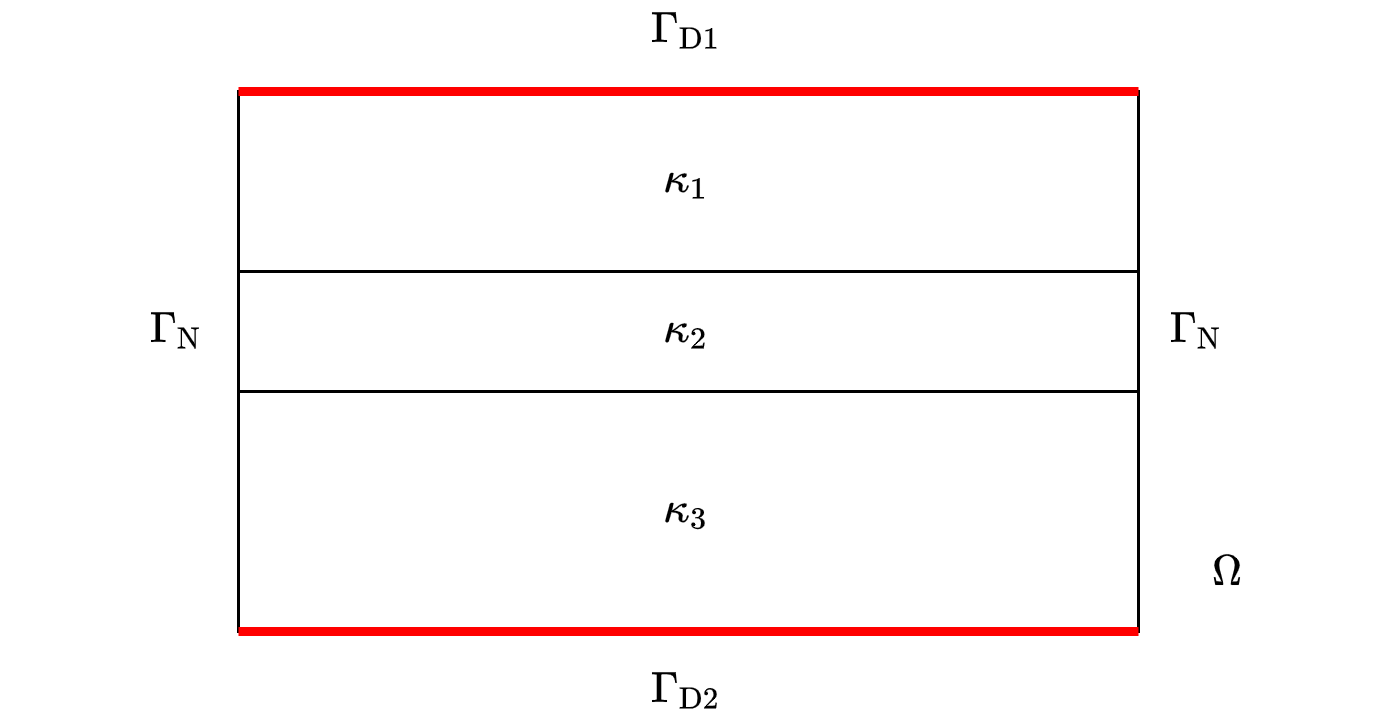
\includegraphics[height=3.5cm]{figures/RBM/Darcy_domain.png}
\end{center}
By the POD, we only need three top singular values and basis functions.
	\begin{figure}[!htbp]
	\centering 
	\includegraphics[width=.36\textwidth]{RBM/singularvalues_3_Darcy.eps}
	\includegraphics[width=.36\textwidth]{RBM/FirstB.png}\\
	\includegraphics[width=.36\textwidth]{RBM/SecondB.png}
	\includegraphics[width=.36\textwidth]{RBM/ThirdB.png}
	\caption{The test problem has three layers of permeability. The distribution of the largest 30 singular values and the basis functions corresponding to the top 3 singular values.}
\end{figure}

Next we approximate $p$ $(\kappa_1=1.55,\kappa_2=1.23,\kappa_3=0.48)$ by model order reduction (MOR).
\begin{figure}[!htbp]
	\centering
	\includegraphics[width=.32\textwidth]{RBM/ph_POD.png}
	\includegraphics[width=.32\textwidth]{RBM/ph_FEM.png}
	\includegraphics[width=.32\textwidth]{RBM/Error_3.png}
	\caption{Comparison of the solutions obtained by MOR and FEM.}
\end{figure}
The computational CPU time is compared as follows: 
\begin{itemize}
	\item FEM: $4.56$s ($64 \times 64$ uniform grid)
	\item MOR online ($d'=3$): $0.0011$s; MOR offline: $327.8$s
\end{itemize}
The reduced model is obtained through offline computation and only one time computation is needed. Given a new $\kappa$, the computational time of using the reduced model is much less than it using FEM.

\paragraph{Efficiency of POD method}
\begin{center}
\includegraphics[width=0.75\textwidth]{RBM/PODtime.png}
\end{center}
From the above table, we have two observations: 
\begin{itemize}
\item Offline step is usually costly
\item If POD works, it can save a lot of online time
\end{itemize}

\subsection{Summary of MOR}
The following figure summarizing the general ideas of MOR
\begin{center}
   \includegraphics[height=4.5cm]{figures/RBM/ROM_Ideas.png}
\end{center}
\begin{itemize}
\item DOF of the reduced model {\color{blue} $d' \ll d$} DOF of the full model
\item Offline computation (costly) can be done just once
\item Online computation (cheap) need to be repeated many times
\end{itemize}

Use POD Eigen-decompostion (or other methods such as greedy algorithm or CNN) to find $\hat{W}$, then do encoder and decoder as follows:

Encoder:
$$
A_{\kappa}x_{\kappa}=b_{\kappa}  \qquad \text{large system in $\mathbb{R}^d$}
$$
$$
\Downarrow f 
$$
%
$$
{\hat{A}_{\kappa}} \hat{x}_{\kappa} = \hat{b}_\kappa \qquad \text{small system in $\mathbb{R}^{d'}$}
$$

Decoder:
$$
x_{\kappa}= g(\hat{x}_{\kappa}) = \hat W \,  \hat{x}_{\kappa} + \bar{x}. 
$$



\section{MOR for time-dependent problem}
\subsection{Model order reduction by POD for time-dependent problem}
There are a lot of complex models in reservoir simulation. To simplify the presentation, we consider the single-phase porous media flow. 
\begin{equation} \label{time-single}
\left\{
\begin{aligned}
\frac{\partial p}{\partial t} - \nabla \cdot (\kappa \nabla p) & = f, & &  [0,T] \times \Omega\\
\kappa \nabla p \cdot n & = 0, & &  [0,T] \times \Gamma_{\text{N}} \\
p & = p_\text{D}, & &  [0,T] \times \Gamma_\text{D} \\
p & = p_{0}, & & \{0\} \times \Omega
\end{aligned}
\right.
\end{equation}
We still FDM discretization for spatial dimension, then we have
\begin{equation}
\frac{\partial x(\kappa, t)}{\partial t}+A_{\kappa}x(\kappa,t)=b_{\kappa}(t).
\end{equation}

\paragraph{Obtain training data}
We generate data $X$ using all snapshots for all parameter samples:
\begin{itemize}
%
\item Pick sample parameters  $\kappa_\ell \in D, \ell=1, 2, \ldots, N$ as we have done for the steady state problem. 
%
\item For each $\kappa_{\ell}$, obtain snapshots at time steps: 
$$
t_m = m \Delta t,\quad  m =1, 2, \ldots, M:=\frac{T}{\Delta t}.
$$
%
\end{itemize}
For each $\kappa$, we solve 
\begin{equation}
\frac{\partial x(\kappa, t)}{\partial t}+A_{\kappa} \, x(\kappa, t)=b_{\kappa}(t)
\end{equation}
using the backward Euler method  
$$
\frac{x(\kappa, t_{m+1})-x(\kappa, t_m)}{\Delta t}+A_{\kappa}x(\kappa,t_{m+1})=b_{\kappa}(t_{m+1})
$$
to obtain 
$$
x ^{m}(\kappa) :=x(\kappa,t_m), \quad m=1,2, \cdots, M \quad \Longrightarrow \quad X_{\kappa} = \Big[x^{1}(\kappa), \ldots, x^{M}(\kappa) \Big].
$$  
Then we have 
$$
X = \Big[ X_{\kappa_{1}}, \ldots, X_{\kappa_{N}} \Big]\in \mathbb{R}^{d\times NM}.
$$

\begin{center}
   \includegraphics[height=5cm]{figures/RBM/TrainingData.png}
\end{center}
We can now apply POD as in the steady-state case to
form $\hat W=[w_1, w_2, \ldots, w_{d'}]\in \mathbb{R}^{d\times d'}$ and we have $\hat W^T\hat W=I_{d'\times d'}$. 

For each new parameter $\kappa\in D$, we only need to solve the reduced problem
\begin{equation}
\frac{\partial  \hat{x}(\kappa, t)}{\partial t}+ \hat{A}_\kappa \, \hat{x}(\kappa,t)  =\hat{b}_{\kappa}(t),
\end{equation}
by the backward Euler method with a new time step size $\Delta \hat t$ which maybe much bigger than $\Delta t$.
Namely 
\begin{equation}
\frac{\hat{x}(\kappa, \hat t_{m+1})-\hat{x}(\kappa, \hat t_{m})}{\Delta \hat t}+\hat{A}_\kappa \, \hat{x}(\kappa, \hat t_{m+1})=\hat{b}_{\kappa}(\hat t_{m+1}).
\end{equation}
Then apply the decoder:
$$
\quad x(\kappa, \hat t_{m+1} )=\hat W \, \hat x(\kappa, \hat t_{m+1}) + \bar{x}. 
$$

\subsection{Numerical results: time-dependent problem}
We still sample 8000 points for $\kappa$, namely, $N=8000$ and set $\Delta t = \frac{1}{256}$, namely, $M=256$, then form the training data $X \in \mathbb{R}^{d \times 2,048,000}$.
\begin{figure}[!htbp]
	\centering 
	\includegraphics[width=.2\textwidth]{figures/POD/singularvalues_Time_Darcy.eps}
	\includegraphics[width=.2\textwidth]{figures/POD/1B.png}
	\includegraphics[width=.2\textwidth]{figures/POD/2B.png}
	\includegraphics[width=.2\textwidth]{figures/POD/3B.png}
	\\
	\includegraphics[width=.2\textwidth]{figures/POD/4B.png}
	\includegraphics[width=.2\textwidth]{figures/POD/5B.png}
	\includegraphics[width=.2\textwidth]{figures/POD/6B.png}
	\includegraphics[width=.2\textwidth]{figures/POD/7B.png}
	\\
	\includegraphics[width=.2\textwidth]{figures/POD/8B.png}
	\includegraphics[width=.2\textwidth]{figures/POD/9B.png}
	\includegraphics[width=.2\textwidth]{figures/POD/10B.png}
	\includegraphics[width=.2\textwidth]{figures/POD/11B.png}
	\\
	\includegraphics[width=.2\textwidth]{figures/POD/12B.png}
	\includegraphics[width=.2\textwidth]{figures/POD/13B.png}
	\includegraphics[width=.2\textwidth]{figures/POD/14B.png}
	\includegraphics[width=.2\textwidth]{figures/POD/15B.png}
	\caption{The basis functions corresponding to the top 15 singular values.}
\end{figure}


Then set $\Delta \hat t=\frac{1}{10}$ and approximate the solution $p$ when $\kappa_1=1.55,\kappa_2=1.23,\kappa_3=0.48$ by MOR.

\begin{center}
%\animategraphics[autoplay,loop,width=0.425\linewidth]{10}{figures/POD/rbm-time-}{0}{9}

\begin{figure}[!htbp]
	\includegraphics[width=.3\textwidth]{figures/POD/ph_POD_time.png}
	\includegraphics[width=.3\textwidth]{figures/POD/ph_FEM_time.png}
	\includegraphics[width=.3\textwidth]{figures/POD/Error_15.png}
	\caption{Comparison of the solutions obtained by MOR and FEM at $t=1$.}
\end{figure}

\end{center}

\subsection{More discussions on Model Order Reduction}
The process of MOR can summarized in the following figure: 
 \begin{center}
     \includegraphics[height=7cm]{figures/RBM/RBM-methods.png}
 \end{center}
\begin{remark} 
If number of parameters is limited, MOR is extremely powerful tool.  We find RBM is useful in many other applications, like FSI  and so on. In fact,  we can apply a greedy algorithm to further reduce offline cost.  For nonlinear problems (with respect to parameters), we can use Empirical Interpolation Method (EIM). However, is it will not work if we have a lot of parameters. 
\end{remark}









































